\section{Progettazione della rete}
\hspace{24pt}Per la realizzazione di questa rete è necessario che ogni host (postazioni e stampanti) abbiano una scheda 
di rete di 1 GBit/s. Tutti gli host presenti al piano terra e al primo piano devono essere forniti di una scheda 
di rete wireless. Per sfruttare al massimo queste schede di rete è necessario che anche gli switch (di piano e non) 
e gli AP abbiano porte da 1 GBit/s. Si ha infine bisogno dei cavi, in questo caso UTP\footnote{Unshielded Twisted Pair} 
di 1 GBit/s di categoria 6, con connettori RJ-45. Tenendo sempre in considerazione la scalabilità e la flessibilità 
della rete, si ha quindi bisogno dei seguenti dispositivi di rete:\\
\begin{itemize}
	\item 7 switch: uno da 4 porte per la sala server, uno da 8 porte per la farmacia del seminterrato, 
	tre da 4 porte per i centri stella di piano e di edificio, due da 8 porte per gli ambulatori
	\item 3 router, per la connessione tra ospedale e ambulatori
	\item 2 AP, per la connessione wireless del piano terra e del primo piano
	\item 15 cavi UTP: 12 per le connessioni host - switch, 3 per le connessioni centro stella 
		  di edificio/piano - router 
\end{itemize}
Supponendo che la direzione dell'ospedale abbia bisogno di una rete veloce e che non abbia "limiti" di budget, i 
collegamenti tra i centri stella di piano e le prese utente, e tra i centri stella di piano e il centro stella di 
edificio saranno realizzati in fibra ottica (FTTH).
Di seguito la rappresentazione grafica della rete.
\vspace*{24pt}
\begin{center}
	\makebox[\textwidth]{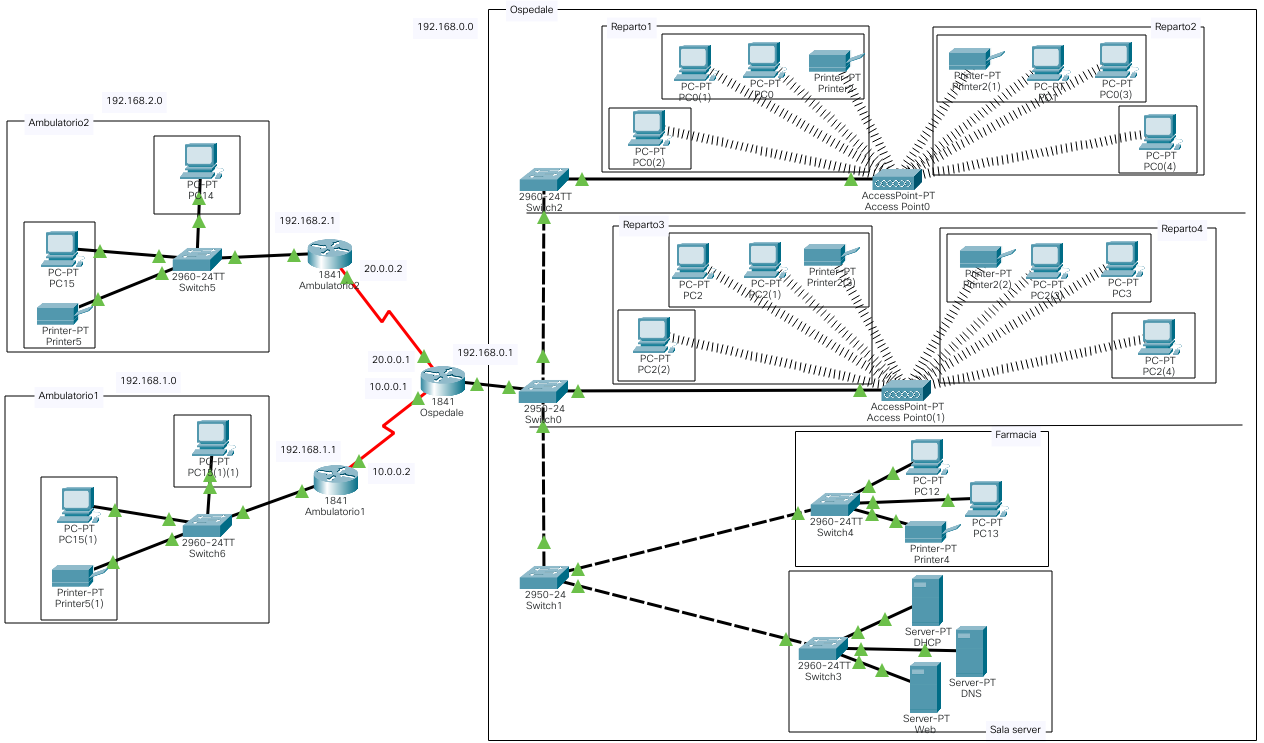
\includegraphics[width=\paperwidth-40pt]{progettazione_rete}}
\end{center}